\documentclass[14pt,a4paper,article]{ncc}
\usepackage[a4paper, mag=1000, left=2.5cm, right=1cm, top=2cm, bottom=2cm, headsep=0.7cm, footskip=1cm]{geometry}
\usepackage[utf8]{inputenc}
\usepackage[T2A]{fontenc}
\usepackage[english,russian]{babel}
\usepackage{indentfirst}
%\usepackage[dvipsnames]{xcolor}
\usepackage{amsfonts} 
\usepackage{amssymb} 
\usepackage{amsmath, etoolbox}
\usepackage{graphicx}
\usepackage{float}
\graphicspath{{../figure/}}
\DeclareGraphicsExtensions{.png,.jpg, .jpeg}

%\bibliographystyle{gost-numeric.bbx}
\usepackage{csquotes}
\usepackage[backend=biber]{biblatex}
\addbibresource{literature.bib}

\usepackage{fancyhdr}
\pagestyle{fancy}
\fancyhead[LE,RO]{\thepage}
\fancyfoot{} 

\usepackage{listings}

%\patchcmd\subequations
%{\theparentequation\alph{equation}}
%{\subequationsformat}
%{}{}

%\newcommand{\subequationsformat}{\theparentequation.\arabic{equation}}

%\numberwithin{equation}{subsection}


\usepackage[colorlinks]{hyperref}
\hypersetup{linkcolor=black}

\begin{document}

% Title page 
\begin{titlepage}
    \begin{center}
        \textsc{
            Санкт-Петербургский политехнический университет Петра Великого \\[5mm]
            Физико-механический институт\\[2mm]
            Высшая школа прикладной математики и вычислительной физики
        }   
        \vfill
        \textbf{\large
            Интервальный анализ\\
            Отчёт по лабораторной работе №1 \\[3mm]
            %по курсовой работе \\[3mm]
        }                
    \end{center}

    \vfill
    \hfill
    \begin{minipage}{0.5\textwidth}
        Выполнил: \\[2mm]   
		Студент: Дамаскинский Константин \\
		Группа: 5040102/10201\\
    \end{minipage}

	\hfill
	\begin{minipage}{0.5\textwidth}
		Принял: \\[2mm]
		к. ф.-м. н., доцент \\   
		Баженов Александр Николаевич
	\end{minipage}

    \vfill
    \begin{center}
        \theyear\ г.
    \end{center}
\end{titlepage}

\tableofcontents
\listoffigures
%\listoftables
\newpage

\section{Постановка задачи}
Проводится исследование из области солнечной энергетики. На рис. 1 показана схема установки для исследования фотоэлектрических характеристик.

\begin{figure}[H]
	\begin{center}
		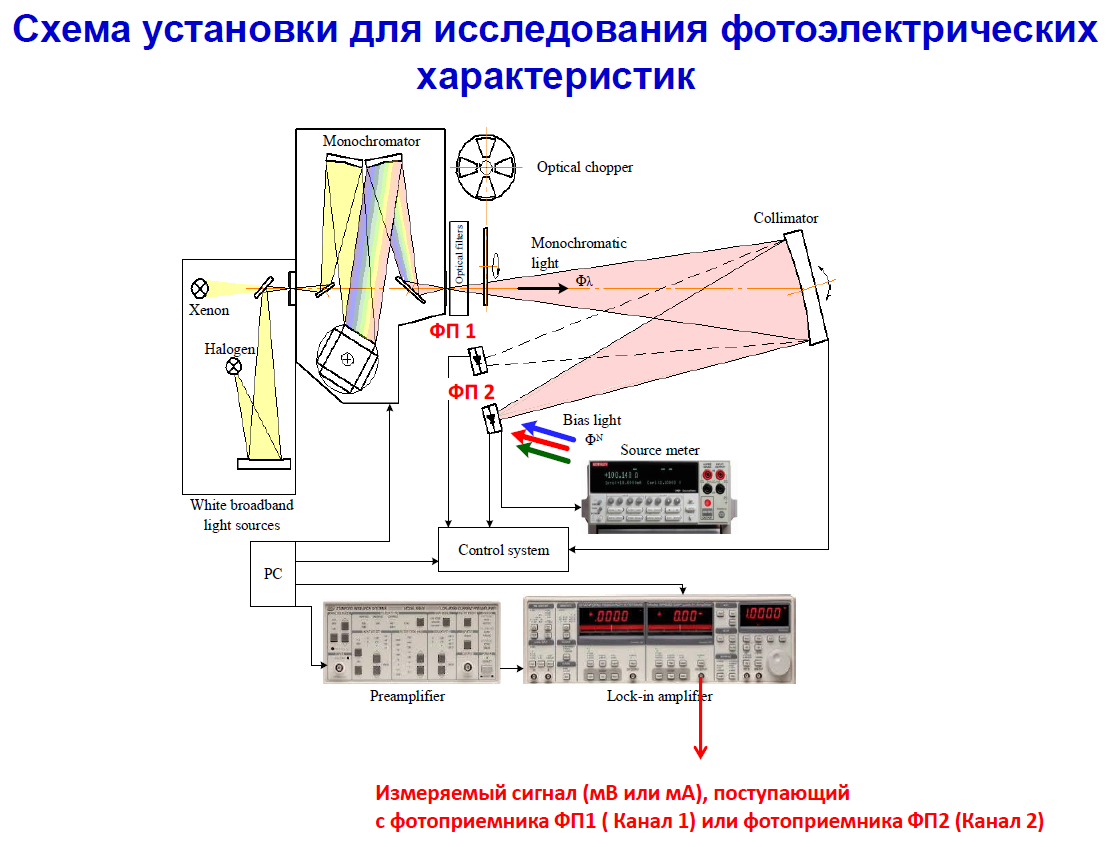
\includegraphics[scale=0.8]{problem1}
		\label{pic:problem1}
		\caption{Схема установки для исследования фотоэлектрических характеристик}
	\end{center}
\end{figure}

Калибровка датчика ФП2 производится по эталону ФП1. Зависимость между квантовыми эффективностями датчиков предполагается постоянной для каждой пары наборов измерений:

\begin{equation}
	QE_2 = \frac{I_2}{I_1} \cdot QE_1
\end{equation}

где $QE_2$, $QE_1$ -- эталонная эффективность эталонного и исследуемого датчика, $I_2$, $I_1$ -- измеренные токи. Данные с датчиков находятся в файлах \textbf{Канал2\_800nm\_0.2.csv}, \textbf{Канал1\_800nm\_0.2.csv} и полагаются линейными.

Требуется определить статус измерений.

\section{Теория}
\subsection{Схема решения задачи}
Будем, как и в прошлой работе, отдельно решать задачу интервальной регресии для двух наборов входных данных $(I, \mathbf{Y_1}), (I, \mathbf{Y_2})$. Здесь $I$ -- номера измерений, $\mathbf{Y_1}, \mathbf{Y_2}$ -- обынтерваленные измеренные значения. В отличие от первой работы, будем решать эти задачи как задачи интервальной, а не вещественной регрессии, описанным ниже способом.

Далее, аналогично предыдущей работе, найдём оптимальный коэффициент $R_{21}$, максимизируя коэффициент Жаккара.

\subsection{Интервальная регрессия как задача оптимизации}
В данной работе для решения задачи интервальной регрессии будем использовать следующий подход.

Будем искать зависимость $y^{(k)} = \beta_0^{(k)} + \beta_1^{(k)}x$ таким образом, чтобы, минимально расширив интервалы исходного интервального вектора $\{\mathbf{y_i}\}_{i=1}^{n}$, получить набор интервалов, накрывающий аппроксимирующую прямую:

\begin{equation} \label{regropt}
\begin{cases}
\mathtt{mid} \mathbf{y^{(k)}_i} - w^{(k)}_i \cdot \mathtt{rad} \mathbf{y^{(k)}_i} \leq \beta_0^{(k)} + \beta_1^{(k)} i \leq \mathtt{mid} \mathbf{y^{(k)}_i} + w^{(k)}_i \cdot \mathtt{rad} \mathbf{y^{(k)}_i} & , \; i = \overline{1, n}\\
\displaystyle\sum_{i=1}^{n} w_i^{(k)} \longrightarrow \min & \\
w_i^{(k)} \geq 0 & , \; i = \overline{1, n} \\
w^{(k)}, \beta_0^{(k)}, \beta_1^{(k)} = ? &
\end{cases}
\end{equation}

Здесь $k \in \{1, 2\}$ -- номер набора данных.

Данная задача является задачей линейного программирования. Как и в прошлой работе, примем $\varepsilon := \mathtt{rad} \mathbf{y_i^{(k)}} = 10^{-4}$ для всех $i = \overline{1, n}$.

\subsection{Информационное множество}

Применительно к данной задаче, информационное множество -- это все такие пары $(\beta_0, \beta_1)$, при которых выполнено первое ограничение типа неравенства задачи оптимизации \ref{regropt}.


\subsection{Коридор совместных зависимостей}

В постановке задаче оптимизации \ref{regropt} не ставится никаких ограничений и целей по минимизации для параметров $\beta_0, \beta_1$. Ясно, что параметры $\beta_0, \beta_1$, полученные в результате решения задачи оптимизации, будут не единственными допустимыми: информационное множество задает целое семейство допустимых $\beta_0, \beta_1$. Следовательно, имеет смысл рассматривать, как единое целое, множество всех функций, совместных с интервальными данными задачи восстановления зависимостей. Такое множество называется \textbf{коридором совместности}.
\textbf{Граничными} называются измерения, определяющие какой-либо фрагмент границы множества. Это свойство имеет смысл рассматривать для наблюдений, принадлежащих выборке, по которой строилась модель. Граничные измерения задают минимальную подвыборку, определяющую модель.

\section{Реализация}
Данная работа реализована на языке программирования Python 3.10 с использованием пакетов numpy и scikitlearn. Код данного отчёта подготовлен с использованием редактора TeXstudio и компилятора pdflatex.

\section{Результаты}
\subsection{Замечания относительно пакета glpk}

Существенный объём времени был потрачен на выяснение причин, по которым пакет glpk не решал задачи, поставленные в модуле ir\_outer.m (минимизация и максимизация $\beta_0$ и $\beta_1$ покомпонентно). Выяснилось, что солвер revised\_simplex не в состоянии найти решения этих задач. Кроме того, солвер interior\_point не мог найти граничные $\beta_0$ и $\beta_1$, когда на переменные не устанавливалось ограничений снизу. После того, как было установлено дефолтное ограничение снизу (т.е 0), interior\_point со всеми задачами успешно справился. В то же время, солвер revised\_simplex в пакете scipy успешно решал те же задачи без искусственных ограничений. Эти проблемы значительно усложнили реализацию данной лабораторной работы, и их, на мой взгляд, следует обнародовать среди студентов.

\subsection{Линейная модель}

Ниже приведены графики, полученные в результате работы реализованной программы.

\begin{figure}[H]
	\begin{center}
		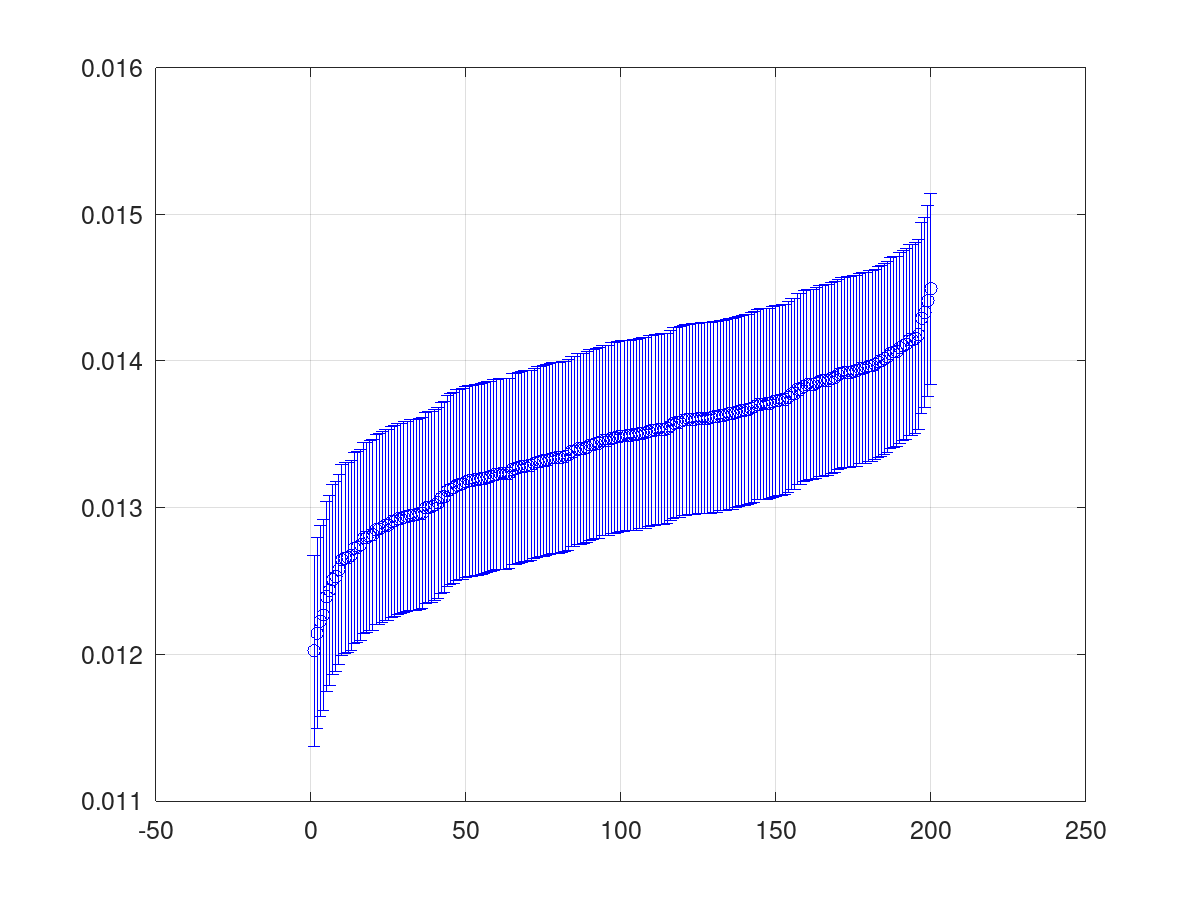
\includegraphics[scale=0.29]{interval_problem_1}
		\label{pic:model1}
		\caption{Обынтерваленные данные. Модель 1}
	\end{center}
\end{figure}

\begin{figure}[H]
	\begin{center}
		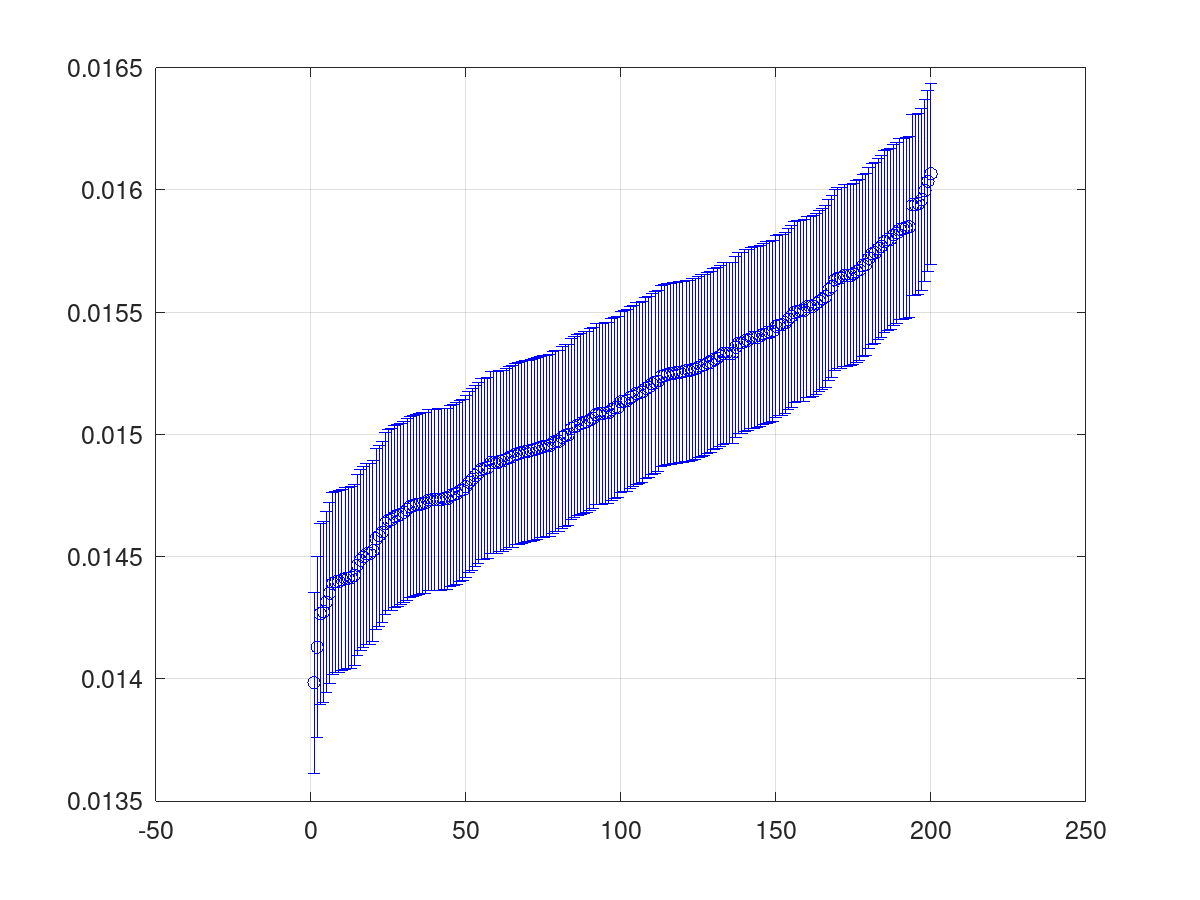
\includegraphics[scale=0.29]{interval_problem_2}
		\label{pic:model2}
		\caption{Обынтерваленные данные. Модель 2}
	\end{center}
\end{figure}

Для ускорения вычислительных процессов и более простого взаимодействия с данными, все интервалы были расширены в максимум из всех полученных весов раз: ширина интервалов составляети $\varepsilon \cdot \max_{i=\overline{1,n}(w_i)}$.

В следующей таблице приведены некоторые отличные от единицы веса:

\begin{table}[H]
	\begin{center}
		\begin{tabular}{|c|c|c|}
			\hline
			Номер интервала & Вес (модель 1) & Вес (модель 2) \\
			\hline
			1 & 6.49 & 3.70 \\
			\hline
			2 & 5.38 & 2.33 \\
			\hline
			3 & 4.63 & 1.04 \\
			\hline
			199 & 2.01 & 1.15  \\
			\hline
			200 & 2.76 & 1.37 \\
			\hline
		\end{tabular}
		\caption{Веса интервалов}
	\end{center}
\end{table}

В обоих случай максимальный вес пришёлся на первый интервал.

В следующей таблице указаны полученные параметры линейной интервальной регрессии (maxdiag).

\begin{table}[H]
	\begin{center}
		\begin{tabular}{|c|c|c|c|}
			\hline
			Модель & $\beta_0$ & $\beta_1$ & $\max w$ \\
			\hline
			1 & 0.012280 & $1.0403 \cdot 10^{-5}$ & 6.49 \\
			\hline
			2 & 0.014142 & $9.3126 \cdot 10^{-6}$ & 3.70 \\
			\hline
		\end{tabular}
		\caption{Параметры линейной интервальной регрессии}
	\end{center}
\end{table}

\begin{figure}[H]
	\begin{center}
		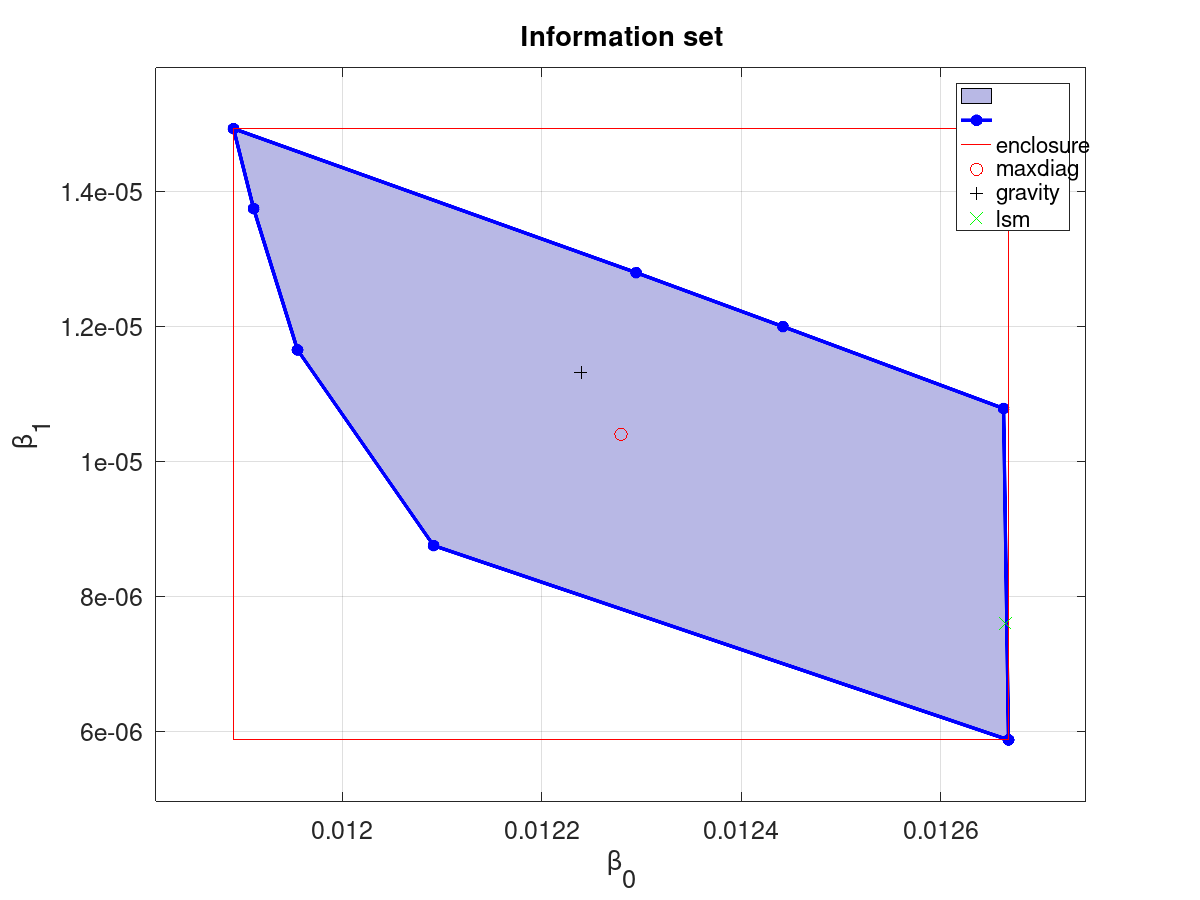
\includegraphics[scale=0.32]{info_set_full_1}
		\label{pic:infoset1}
		\caption{Информационное множество. Модель 1}
	\end{center}
\end{figure}

\begin{figure}[H]
	\begin{center}
		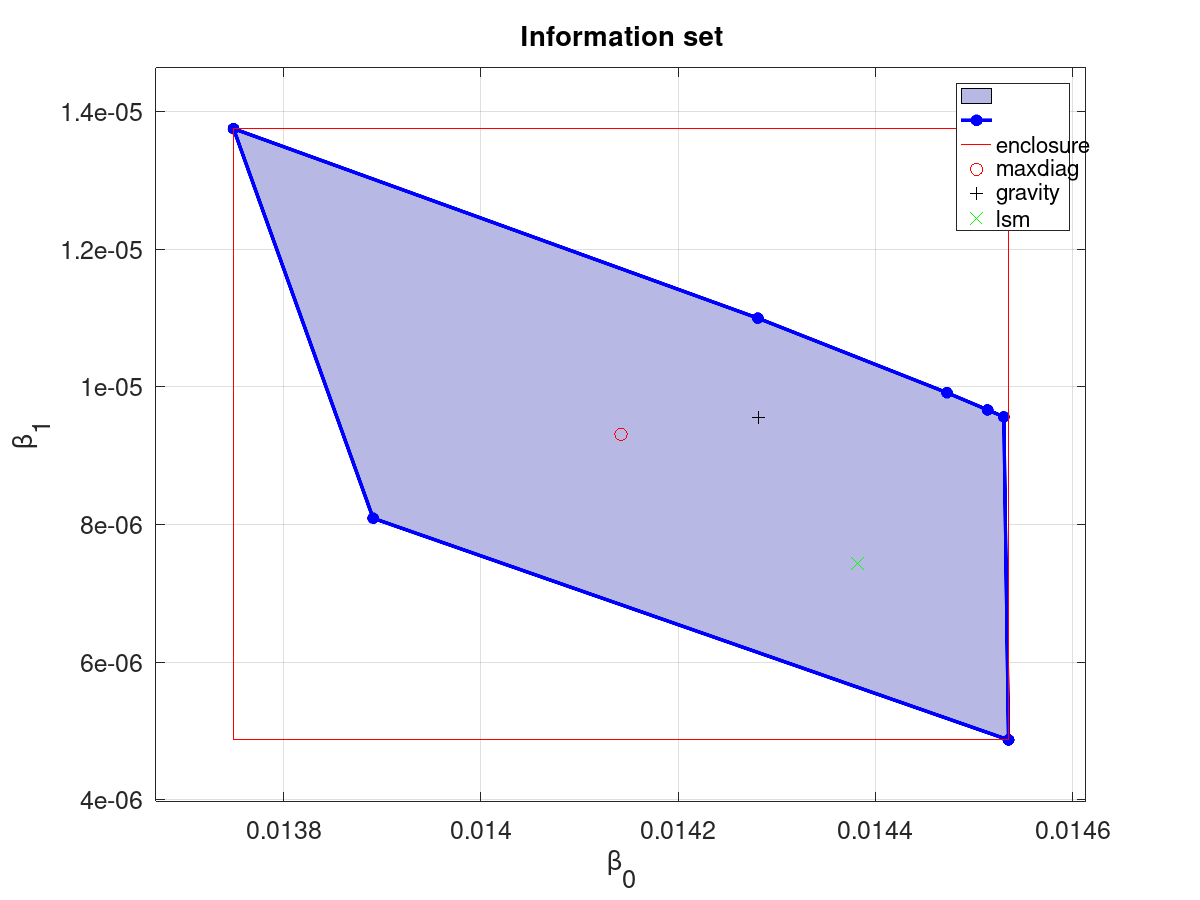
\includegraphics[scale=0.32]{info_set_full_2}
		\label{pic:infoset2}
		\caption{Информационное множество. Модель 2}
	\end{center}
\end{figure}

\begin{figure}[H]
	\begin{center}
		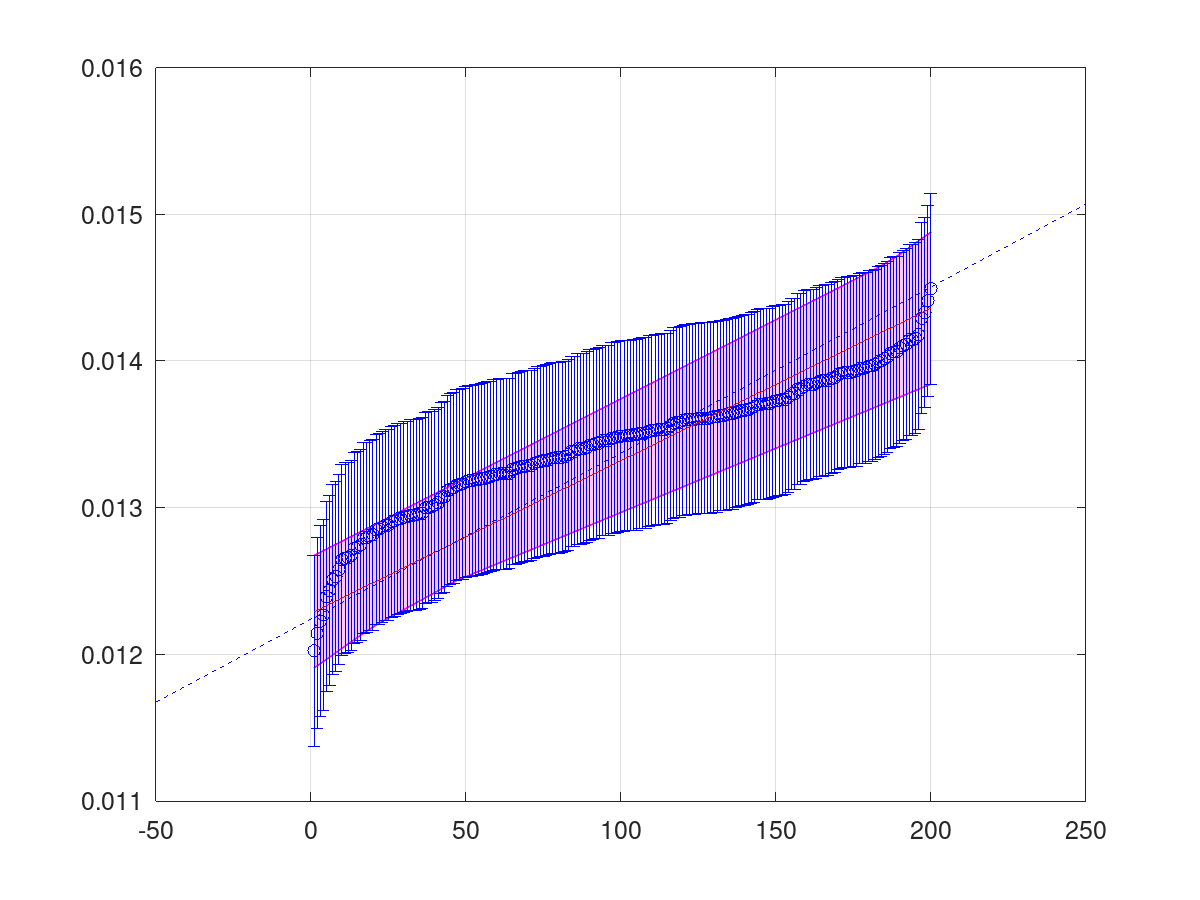
\includegraphics[scale=0.32]{joint_depth_1}
		\label{pic:joint_depth1}
		\caption{Коридор совместных зависимостей. Модель 1}
	\end{center}
\end{figure}

\begin{figure}[H]
	\begin{center}
		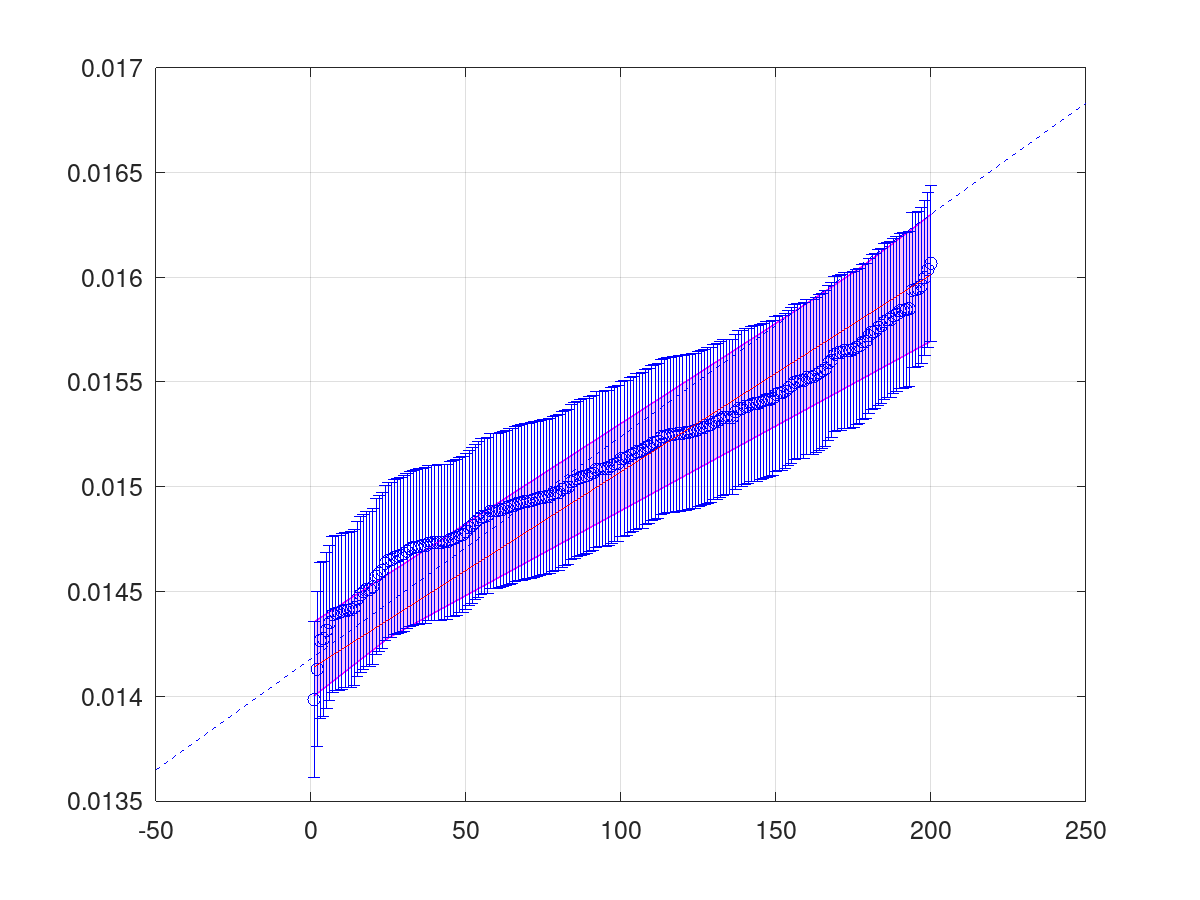
\includegraphics[scale=0.32]{joint_depth_2}
		\label{pic:joint_depth2}
		\caption{Коридор совместных зависимостей. Модель 2}
	\end{center}
\end{figure}

\begin{figure}[H]
	\begin{center}
		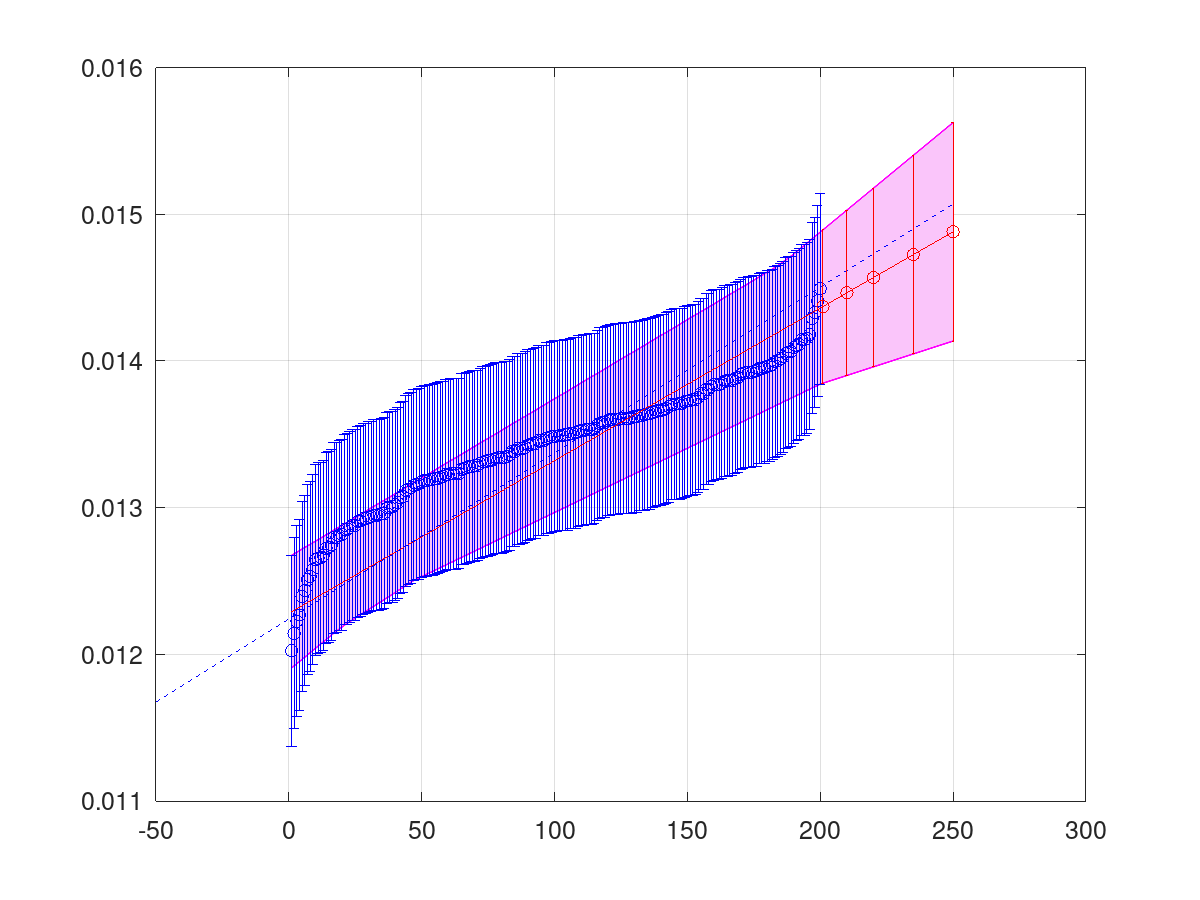
\includegraphics[scale=0.32]{prediction_1}
		\label{pic:prediction1}
		\caption{Коридор совместных зависимостей. Предсказанные значения. Модель 1}
	\end{center}
\end{figure}

\begin{figure}[H]
	\begin{center}
		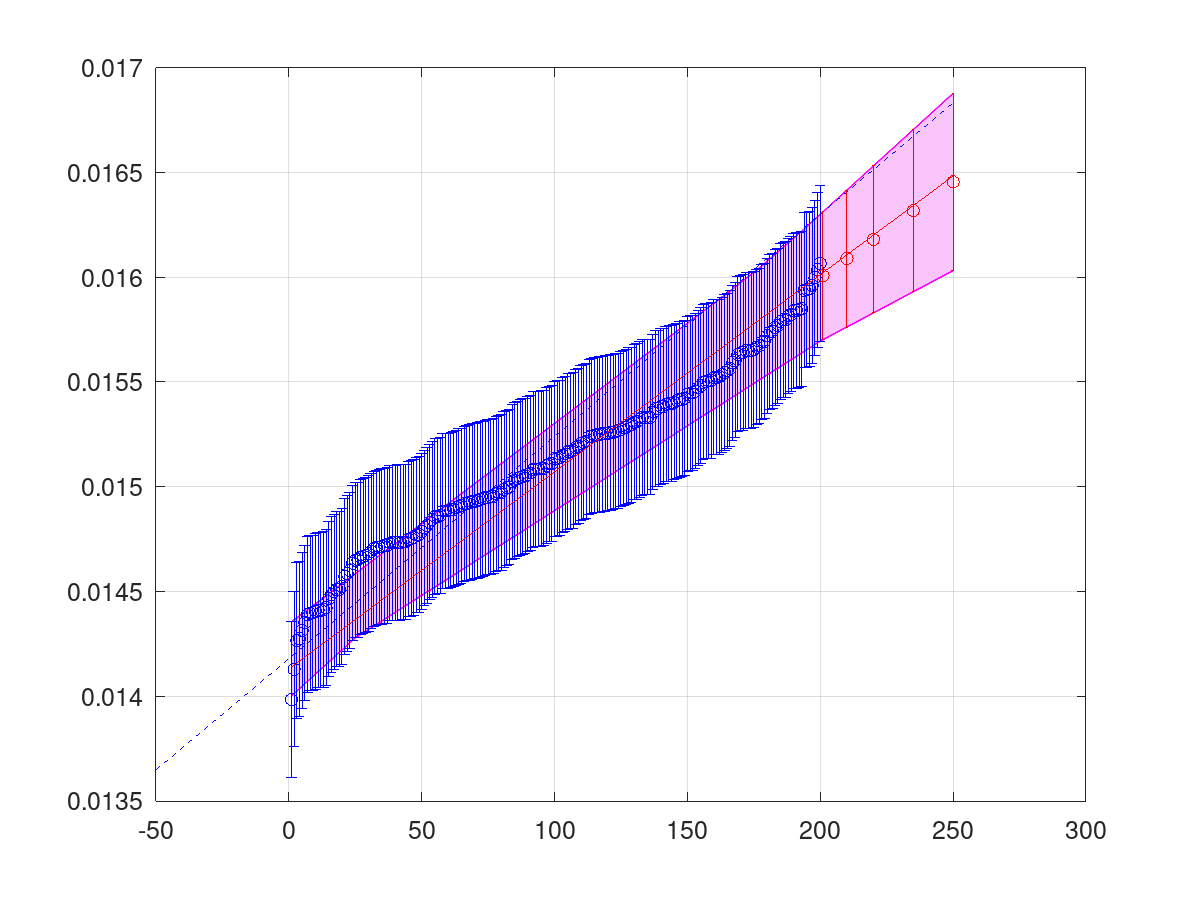
\includegraphics[scale=0.32]{prediction_2}
		\label{pic:prediction2}
		\caption{Коридор совместных зависимостей. Предсказанные значения. Модель 2}
	\end{center}
\end{figure}

Граничные точки в первой модели -- точки под номерами 1, 17, 21, 47, 182, 184, 189, 200.

Граничные точки во второй модели -- 1, 25, 162, 165, 177, 193, 200.


Максимальный коэффициент Жаккара, рассчитанный прежним методом при параметрах $\beta_0, \beta_1$, полученных как точка пересечения максимальных диагоналей (maxdiag) оказался равен 0.0615, в то время как в прошлой реализации он равен 0.037, что в 1.65 раз выше. Оптимальный коэффициент $R_{21}$ в таком случае равен 0.882, что отличается от прошлого варианта на 0.003.

\begin{figure}[H]
	\begin{center}
		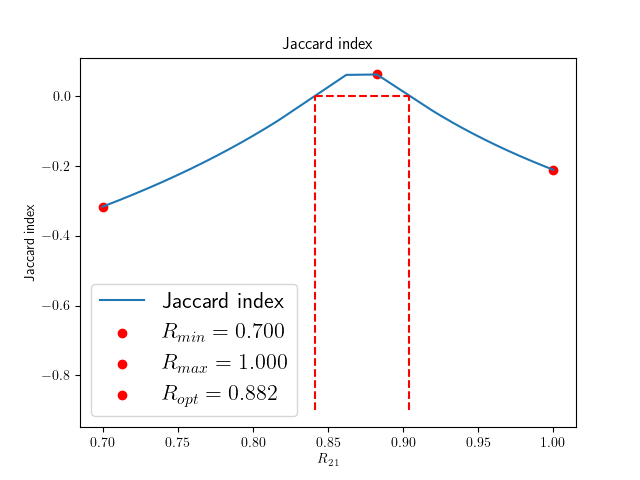
\includegraphics[scale=0.52]{jaccard}
		\label{pic:jaccard}
		\caption{Зависимость коэффициента Жаккара от множителя $R_{21}$}
	\end{center}
\end{figure}

\subsection{Кусочно-линейная модель}

Далее была произведена процедура кусочно-линейной интервальной регрессии: выше описанная процедура была проделана для трёх отдельных участков данных: 1-50, 51-150, 151-200. В результате были получены следующие параметры регрессии:

\begin{table}[H]
	\begin{center}
		\begin{tabular}{|c|c|c|c|}
			\hline
			Диапазон & $\beta_0$ & $\beta_1$ & $\max w$ \\
			\hline
			1-50 & 0.01217 & $2.0065 \cdot 10^{-5}$ & 6.54 \\
			\hline
			51-150 & 0.01269 & $7.4948 \cdot 10^{-6}$ & 1.00 \\
			\hline
			151-200 & 0.01149 & $1.471 \cdot 10^{-5}$ & 1.67 \\
			\hline
		\end{tabular}
		\caption{Параметры кусочно-линейной интервальной регрессии. Модель 1}
	\end{center}
\end{table}

\begin{table}[H]
	\begin{center}
		\begin{tabular}{|c|c|c|c|}
			\hline
			Диапазон & $\beta_0$ & $\beta_1$ & $\max w$ \\
			\hline
			1-50 & 0.01420 & $1.368 \cdot 10^{-5}$ & 2.31 \\
			\hline
			51-150 & 0.01431 & $8.109 \cdot 10^{-6}$ & 1.00 \\
			\hline
			151-200 & 0.01318 & $1.431 \cdot 10^{-5}$ & 1.00 \\
			\hline
		\end{tabular}
		\caption{Параметры кусочно-линейной интервальной регрессии. Модель 2}
	\end{center}
\end{table}

Обынтерваленные данные выглядят следующим образом:

\begin{figure}[H]
	\begin{center}
		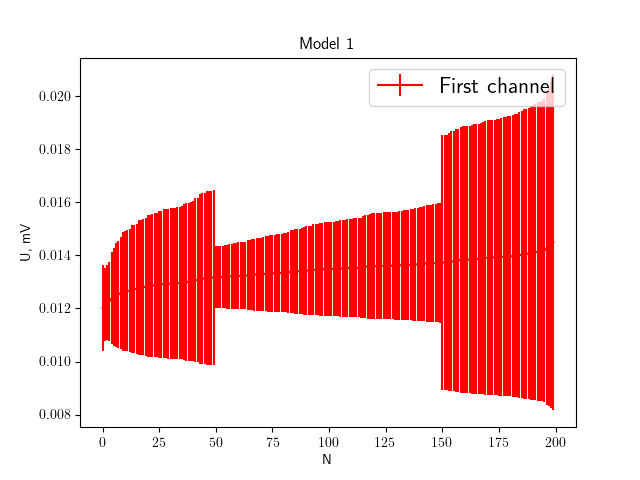
\includegraphics[scale=0.72]{partial1}
		\label{pic:part1}
		\caption{Кусочно-линейная регрессия. Модель 1}
	\end{center}
\end{figure}

\begin{figure}[H]
	\begin{center}
		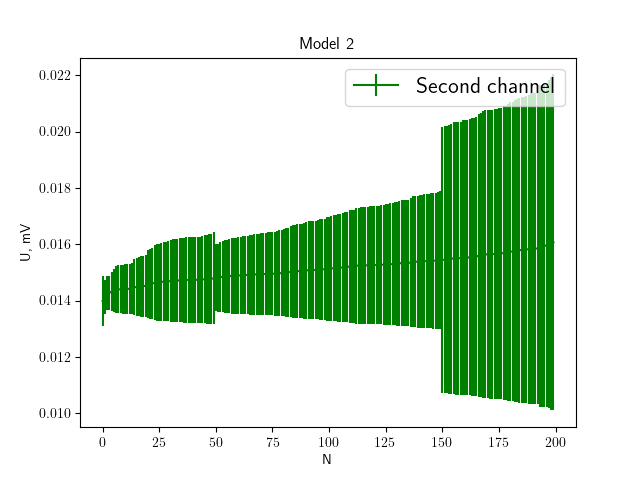
\includegraphics[scale=0.72]{partial2}
		\label{pic:part2}
		\caption{Кусочно-линейная регрессия. Модель 2}
	\end{center}
\end{figure}

При построении кусочно-линейной регрессии удалось добиться коэффициента Жаккара, равного 0.0667, что на 0.0052 больше, чем в случае линейной интервальной регрессии. Примечательно, что оптимальный множитель $R_{21}$ в таком случае оказался равен 0.888: линейная регрессия дала отклонение коэффициента влево от точечной на 0.003, а кусочно-линейная -- вправо на то же значение.

\begin{figure}[H]
	\begin{center}
		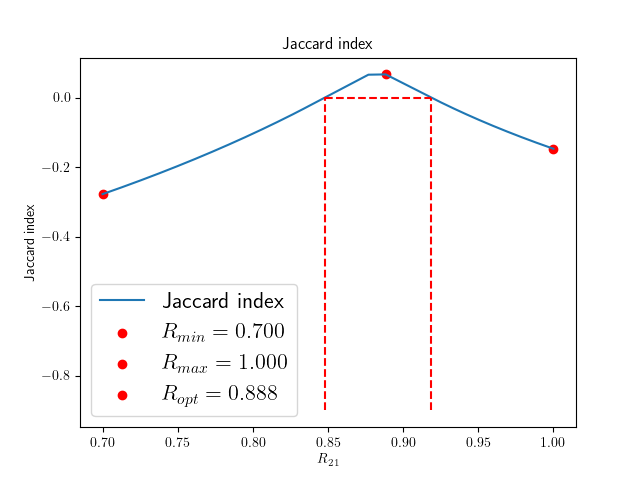
\includegraphics[scale=0.75]{jaccard_partial}
		\label{pic:jaccard2}
		\caption{Зависимость коэффициента Жаккара от множителя $R_{21}$}
	\end{center}
\end{figure}


\section{Обсуждение}

Видно, что точки из центральной части, как и ожидается, лежат в зелёной зоне. Чем больше увеличивается ширина интервалов, тем больше точек из левой и правой части попадают в зелёную зону. При радиусе в $6 \cdot 10 ^ {-4}$ в обоих выборках точки из всех трёх частей попадают в зелёную зону.
Также видно, что строго внешние измерения встречаются только во второй выборке при радиусе интервала $10 ^ {-4}$, а выбросы были обнаружены при том же радиусе в первой выборке.

\printbibliography
%\addcontentsline{toc}{section}{Литература}

\section{Приложения} \label{app}

\begin{enumerate}
	\item Репозиторий с кодом программы и кодом отчёта:
	
	\href{https://github.com/kystyn/interval}{https://github.com/kystyn/interval2}

\end{enumerate}

\end{document}
